\parindent=0em
\section{Shader de profundidad}
\noindent

Un \textit{shader}~\cite{thebookofshaders} se puede definir como un programa que se ejecuta en la GPU y procesa todos los píxeles de la pantalla uno a uno en cada \textit{frame}, este programa se puede implementar en diferentes lenguajes de \textit{shading} como por ejemplo GLSL y se utiliza con el objetivo de aplicar efectos de post-procesado (modificando el color, tono, brillo... de cada píxel). Además, gracias a los \textit{shaders} se pude aplicar distintos efectos a los objetos 3D o imágenes de una escena como ruido (figura~\ref{fig:shadernoise}) o efecto de pintura entre muchos otros.

\begin{figure}[htbp]
\centering
    \hspace{-4mm}
    \begin{minipage}{0.5\textwidth}
        \centering
        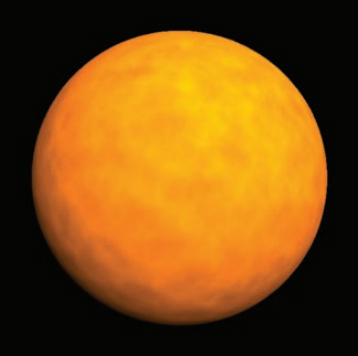
\includegraphics[scale=0.5]{Images/Shaders/luna1.jpg}\\
    \end{minipage}
    \begin{minipage}{0.5\textwidth}
        \centering
        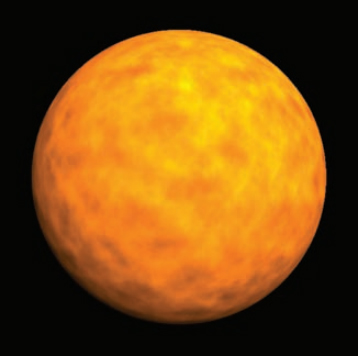
\includegraphics[scale=0.5]{Images/Shaders/luna2.jpg}\\
    \end{minipage}\\
    \caption[Distintos tipos de ruido aplicados como texturas a una esfera]{Distintos tipos de ruido aplicados como texturas a una esfera\footnotemark.}
    \label{fig:shadernoise}
\end{figure}

\footnotetext{Fuente: Graphics Shaders: Theory and Practice~\cite{grapchisshaderstheory}}

En primer lugar, con el objetivo de crear un mapa de calor para realizar un efecto de oclusión, se creó un \textit{shader} en Unity (donde para implementar \textit{shaders} se utiliza una combinación de los lenguajes HLSL y Cg) que afectase a la transparencia de los objetos en función de su profundidad (detectada por ARCore).\\

%https://docs.unity3d.com/Manual/SL-CameraDepthTexture.html

Este \textit{shader} utilizaba la textura de profundidad que genera la cámara de Unity\footnotemark, con esa información, se le aplicaba a los objetos un material con una variable ``DepthLevel'' la cual contenía el valor de profundidad obtenido en la textura generada por la cámara, este valor modificaba el valor de transparencia del objeto. En primer lugar se hizo una prueba del \textit{shader} con un cubo que podía acercarse y alejarse con unos botones, como se puede observar en la figura~\ref{fig:shaderprofprueba1}, el valor de transparencia del cubo se ve afectado en función de su profundidad respecto al dispositivo.\\

\footnotetext{Textura de profundidad de Unity: \url{https://docs.unity3d.com/Manual/SL-CameraDepthTexture.html}}

Dicho cubo era un elemento fijado a la cámara, es decir, seguía su movimiento, además, el \textit{shader} se le aplicaba a todos los elementos de la escena que poseían el material que tenía la variable de profundidad mencionada anteriormente. Aunque lo más común es aplicar el \textit{shader} a un material concreto, ya que este utilizaba la textura de profundidad de la cámara estaba aplicado a ella.\\

En resumen, la cámara generaba una textura de profundidad en cada \textit{frame} donde se modificaba el valor de transparencia de los objetos que estuviesen dotados de un material en concreto, generando mayor transparencia a mayor profundidad.

\begin{figure}[htbp]
\centering
    \hspace{-4mm}
    \begin{minipage}{0.3\textwidth}
        \centering
        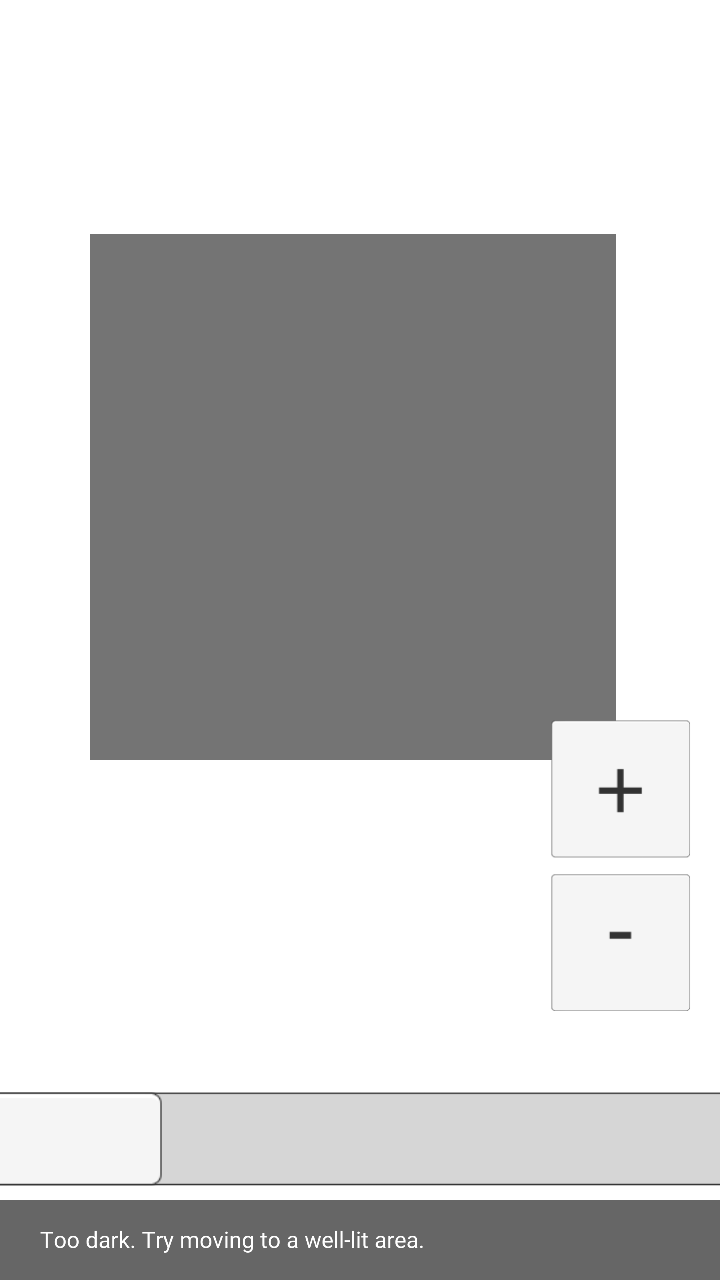
\includegraphics[scale=0.15]{Images/Shaders/profundidad (1).png}\\
    \end{minipage}
    \begin{minipage}{0.3\textwidth}
        \centering
        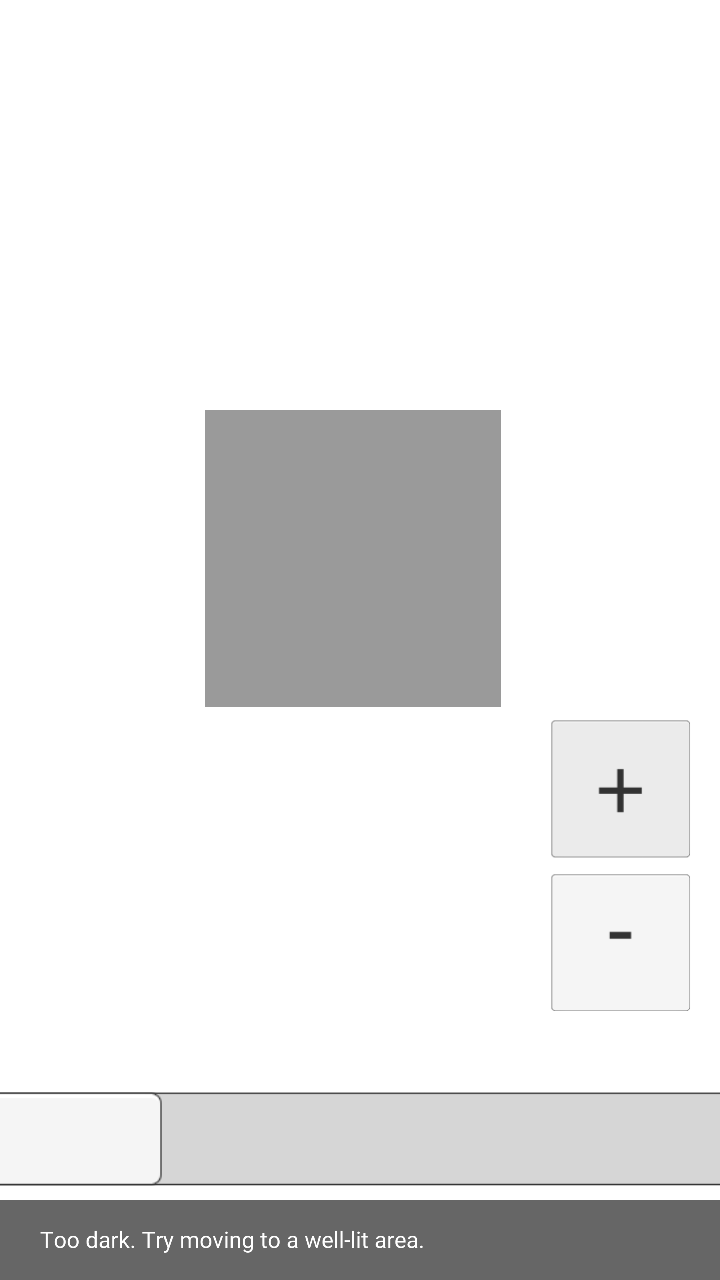
\includegraphics[scale=0.15]{Images/Shaders/profundidad (2).png}\\
    \end{minipage}
    \begin{minipage}{0.3\textwidth}
        \centering
        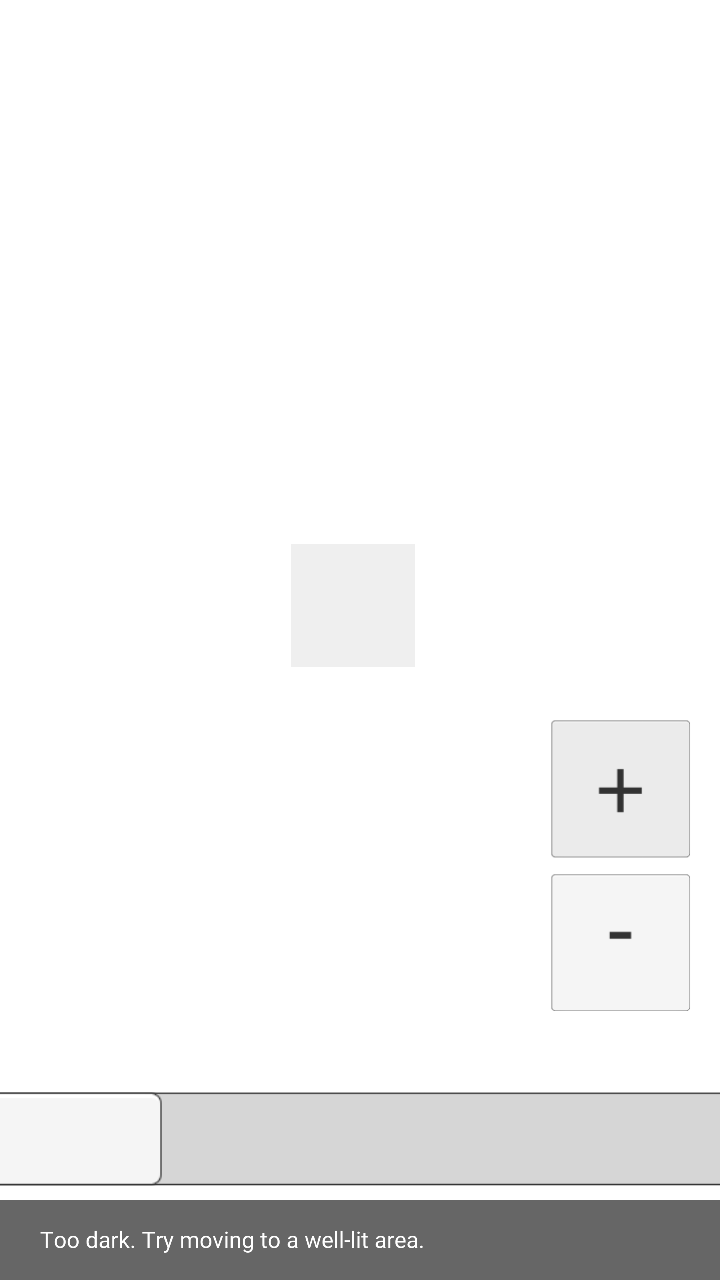
\includegraphics[scale=0.15]{Images/Shaders/profundidad (3).png}\\
    \end{minipage}\\
    \caption[\textit{Shader} de profundidad aplicado a un cubo con profundidad variable]{\textit{Shader} de profundidad aplicado a un cubo con profundidad variable.}
    \label{fig:shaderprofprueba1}
\end{figure}

Como esta prueba había sido exitosa y el objetivo final del \textit{shader} era generar un mapa de calor basado en la profundidad, se intentó aplicar este efecto de post-procesado a la nube de puntos (punto~\ref{sec:nubeDePuntos}) generada por ARCore. Se llegó a la conclusión de que este \textit{shader}, al ser un efecto que modificaba la textura de la cámara, no se aplicaba a la nube de puntos obteniendo los resultados de la figura~\ref{fig:shaderprofp2} donde se aprecia que se está modificando la transparencia del cubo pero no de los puntos generados por ARCore.

\begin{figure}[H]
\centering
    \hspace{-4mm}
    \begin{minipage}{0.5\textwidth}
        \centering
        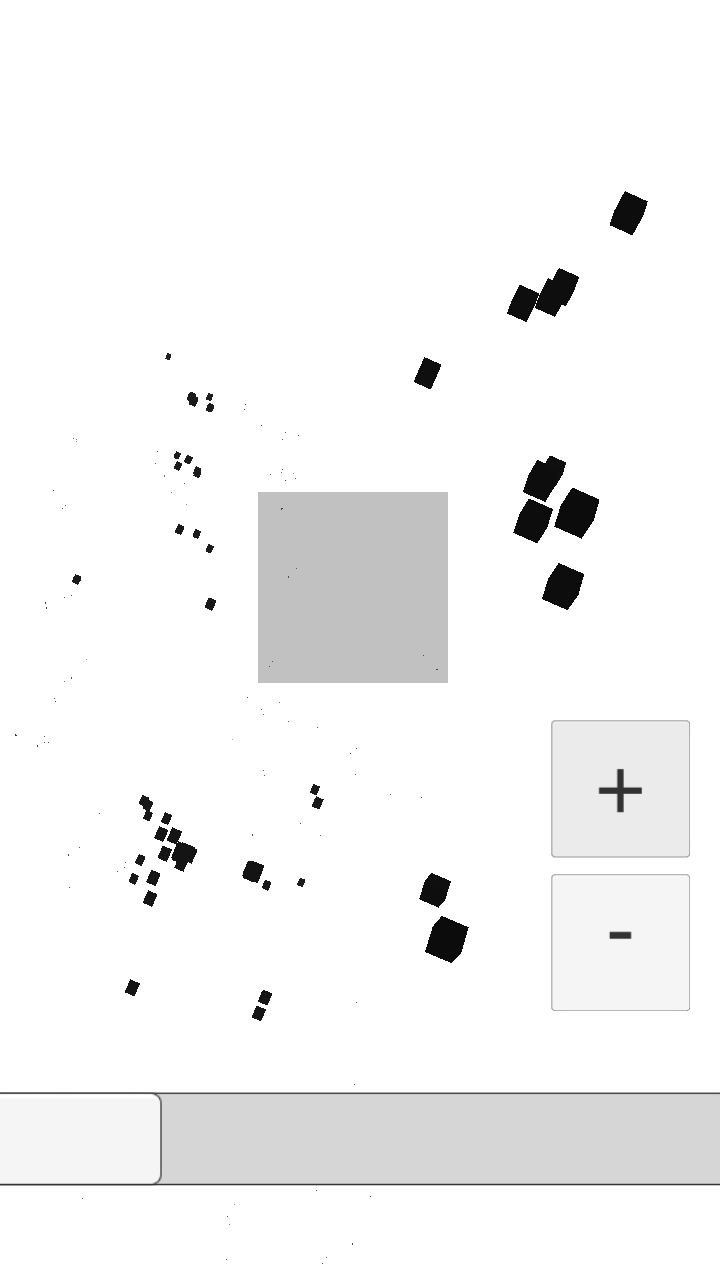
\includegraphics[scale=0.2]{Images/Shaders/profundidad (4).png}\\
    \end{minipage}
    \begin{minipage}{0.5\textwidth}
        \centering
        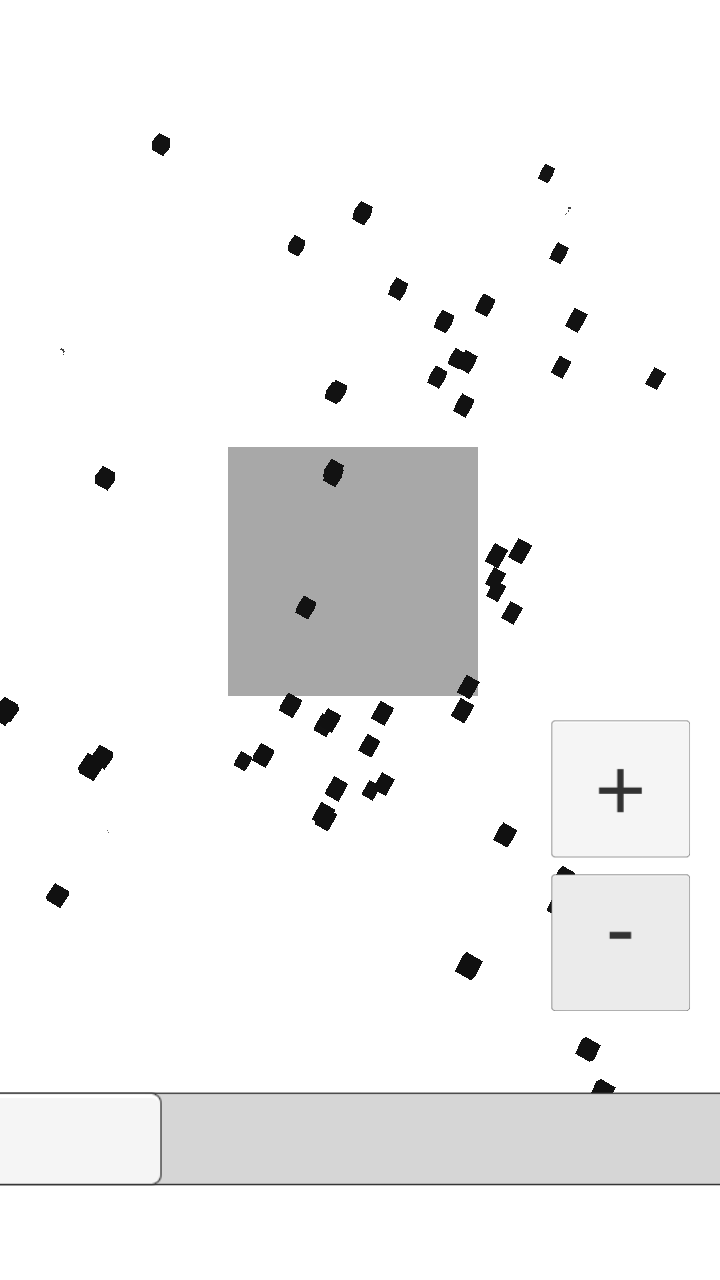
\includegraphics[scale=0.2]{Images/Shaders/profundidad (5).png}\\
    \end{minipage}\\
    \caption[\textit{Shader} de profundidad modificando el cubo pero no la nube de puntos]{\textit{Shader} de profundidad modificando el cubo pero no la nube de puntos.}
    \label{fig:shaderprofp2}
\end{figure}

Debido a estos resultados se descartó este efecto de post-procesado y se pasó a contemplar otras alternativas. 